\documentclass[11pt]{article}
\usepackage[top=1cm, bottom=2cm, left=1cm, right=1cm]{geometry}
\usepackage{ctex}
\usepackage{float}
\usepackage{algorithm}
\usepackage{algorithmicx}
\usepackage{algpseudocode}
\usepackage{amsthm,amsmath,amssymb}
\usepackage[colorlinks=true,linkcolor=blue]{hyperref}
\usepackage{listings}
\usepackage{xcolor,xparse}
\usepackage{realboxes}
\usepackage{graphics}
\usepackage{graphicx}
\usepackage{mathrsfs}
\usepackage{wrapfig}
\usepackage{subfigure}
\usepackage{pifont}

\definecolor{cmdbg}{rgb}{0.9,0.9,0.9}
\lstset{%
	basicstyle=\ttfamily,
	breaklines = true,
	backgroundcolor=\color{cmdbg},
}
\DeclareDocumentCommand{\ccmd}{v}{% 参数 v 表示工作方法类似于 \verb
    \Colorbox{cmdbg}{\csname lstinline\endcsname!#1!}%
}

\makeatletter
\newenvironment{breakablealgorithm}
  {% \begin{breakablealgorithm}
   \begin{center}
     \refstepcounter{algorithm}% New algorithm
     \hrule height.8pt depth0pt \kern2pt% \@fs@pre for \@fs@ruled
     \renewcommand{\caption}[2][\relax]{% Make a new \caption
       {\raggedright\textbf{\ALG@name~\thealgorithm} ##2\par}%
       \ifx\relax##1\relax % #1 is \relax
         \addcontentsline{loa}{algorithm}{\protect\numberline{\thealgorithm}##2}%
       \else % #1 is not \relax
         \addcontentsline{loa}{algorithm}{\protect\numberline{\thealgorithm}##1}%
       \fi
       \kern2pt\hrule\kern2pt
     }
  }{% \end{breakablealgorithm}
     \kern2pt\hrule\relax% \@fs@post for \@fs@ruled
   \end{center}
  }
\makeatother

\author{李明钰 22307110156}
\title{计算物理作业n}

\begin{document}
\maketitle


\section{题目1:太阳黑子数据处理}
\subsection{题目描述}
Detecting periodicity: Download the file called sunspots.txt , which contains the observed number of sunspots on the Sun for each month since January 1749. Write a program to calculate the Fourier transform of the sunspot data and then make a graph of the magnitude squared $|c_k|^2$
 of the Fourier coefficients as a function of k
 —also called the power spectrum of the sunspot signal. You should see that there is a noticeable peak in the power spectrum at a nonzero value of k
. Find the approximate value of k
 to which the peak corresponds. What is the period of the sine wave with this value of k?

%\begin{wrapfigure}{r}{0.4\textwidth}
%图片

\subsection{程序描述}
先使用numpy(以下简称np)读取sunspots.txt文件,将其月份数据和对应的太阳黑子数数据分别存入两个数组中,随后用算法\ref{FFT}分析得到其周期。
\subsection{伪代码}
高斯消去法的伪代码如下所示
\begin{breakablealgorithm}
    \caption{FFT分析太阳黑子周期}
    \label{FFT}
\begin{algorithmic}[1]
\REQUIRE Sunspot data array: $\text{sunspot\_data}$ (monthly sunspot counts since January 1749)
\ENSURE Period of the dominant sine wave in months: $\text{period\_in\_months}$

\STATE \textbf{Step 1: Compute Fourier coefficients}
\STATE $\text{fft\_coeffs} \gets \text{FFT}(\text{sunspot\_data})$ 
\COMMENT{Perform Fourier transform to decompose the time series into frequency components.}

\STATE \textbf{Step 2: Compute frequencies associated with Fourier coefficients}
\STATE $\text{frequencies} \gets \text{FFTFreq}(\text{len}(\text{sunspot\_data}), d=1)$
\COMMENT{Calculate the corresponding frequencies for each Fourier coefficient, assuming a sampling interval of 1 month.}

\STATE \textbf{Step 3: Compute the power spectrum}
\STATE $\text{power\_spectrum} \gets |\text{fft\_coeffs}|^2$
\COMMENT{The power spectrum quantifies the contribution of each frequency to the overall signal.}

\STATE \textbf{Step 4: Filter out zero-frequency components (DC component)}
\STATE $\text{nonzero\_freqs} \gets \text{frequencies}[\text{frequencies} > 0]$
\STATE $\text{nonzero\_power} \gets \text{power\_spectrum}[\text{frequencies} > 0]$
\COMMENT{Exclude the zero frequency component to focus on periodic variations.}

\STATE \textbf{Step 5: Identify the peak in the power spectrum}
\STATE $\text{peak\_index} \gets \text{argmax}(\text{nonzero\_power})$
\COMMENT{Find the index of the highest peak in the power spectrum, indicating the dominant frequency.}

\STATE \textbf{Step 6: Find the corresponding frequency of the peak}
\STATE $\text{peak\_frequency} \gets \text{nonzero\_freqs}[\text{peak\_index}]$
\COMMENT{Retrieve the frequency associated with the dominant peak.}

\STATE \textbf{Step 7: Calculate the period of the sine wave}
\STATE $\text{period\_in\_months} \gets \frac{1}{\text{peak\_frequency}}$
\COMMENT{Convert the frequency to the period, representing the cycle length in months.}

\RETURN $\text{period\_in\_months}$
\COMMENT{Output the period of the dominant sine wave.}
\end{algorithmic}
\end{breakablealgorithm}

\subsection{输入输出实例}
原始数据如下图所示
\begin{figure}[H]
    \centering
    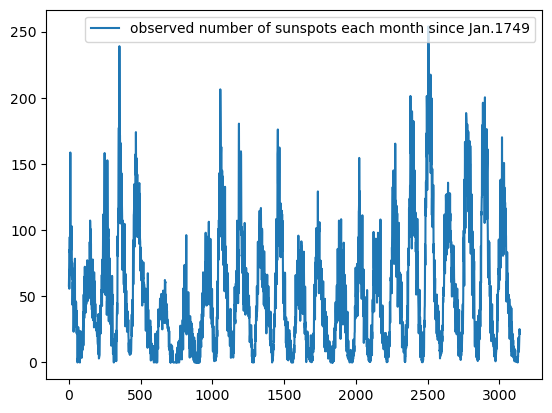
\includegraphics[width=0.5\linewidth]{data.png}
    \caption{太阳黑子数随月份变化关系}
    \label{fig:太阳黑子数随月份变化关系}
\end{figure}

经过快速傅里叶变换得到结果如图所示
\begin{figure}[H]
    \centering
    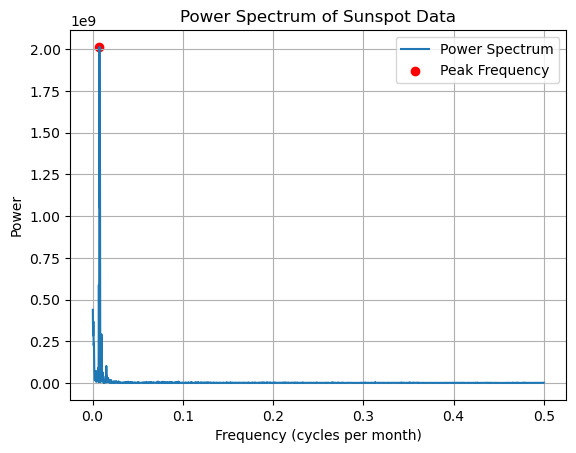
\includegraphics[width=0.5\linewidth]{output.png}
    \caption{快速傅里叶变换结果}
    \label{fig:快速傅里叶变换结果}
\end{figure}

因此得到结论为
\begin{figure}[H]
    \centering
    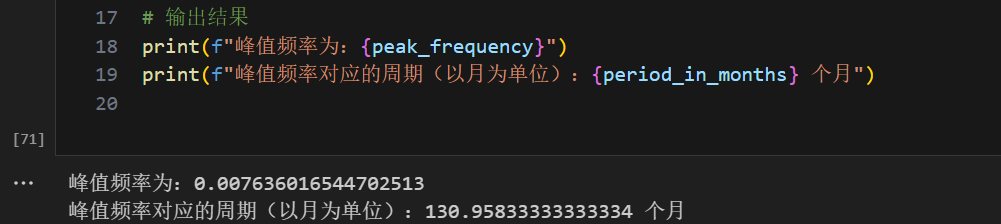
\includegraphics[width=0.5\linewidth]{conclusion.png}
    \caption{分析结论}
    \label{fig:分析结论}
\end{figure}

%\begin{figure}[ht]


\end{document}
